\documentclass{article}

\usepackage{homework}

%
% 封面信息设置
%
\renewcommand{\hmwkTitle}{Catch Turtle All}
\renewcommand{\hmwkSubTitle}{Group4 Project Report}
\renewcommand{\hmwkClass}{《ROS2机器人开发》}
\renewcommand{\hmwkClassInstructor}{}
\renewcommand{\hmwkAuthorName}{LAOSIKAI 50091097}
\renewcommand{\hmwMajor}{Computer Science}
\renewcommand{\hmwNumber}{}

\title{
	
\includegraphics[scale = 0.45]{logo.jpg}\\
    \vspace{1in}
    \textmd{\textbf{\hmwkTitle\ }}\\
   \textmd{\textbf{\hmwkSubTitle}}\\
    \vspace{0.1in}\large{\textit{\hmwkClassInstructor\ }}\\
            \vspace{3in}
    \hmwMajor{}\\
    \hmwkAuthorName{}\\
}

\date{\today}

%
% 正文部分
%
\begin{document}

\maketitle

\tableofcontents

\pagebreak

%=============================================================================
% Chapter 1: Project Overview and Objectives
%=============================================================================
\begin{homeworkProblem}[1]
\section{Chapter 1: Project Overview and Objectives}

\subsection{Project Overview}

The \textbf{Catch Turtle All} project is a ROS2-based robotic simulation system that demonstrates autonomous pursuit, task scheduling, and formation following within the \texttt{turtlesim} environment. Built on ROS2 Humble with Python, the system orchestrates multiple cooperating nodes to create a dynamic, self-sustaining multi-agent scenario.

The core concept is straightforward: a master turtle (\texttt{turtle1}) continuously hunts newly spawned target turtles across the simulation canvas. Once a target is caught, it joins a following chain behind the master, forming an ever-growing snake-like formation. New targets are generated periodically, ensuring the system never runs out of objectives.

The system consists of five ROS2 nodes organised in a layered architecture: \texttt{turtlesim\_node} (simulation), \texttt{spawn\_manager} (environment generation), \texttt{master\_manager} (task management), \texttt{catch\_executor} (execution control), and \texttt{follower\_manager} (formation following). The operational loop is: \textit{spawn targets} $\rightarrow$ \textit{discover and track} $\rightarrow$ \textit{select nearest} $\rightarrow$ \textit{pursue via Action} $\rightarrow$ \textit{catch and add to chain} $\rightarrow$ \textit{repeat}.

\subsection{Project Objectives}

The project is designed to achieve the following objectives:

\begin{enumerate}[label=\textbf{O\arabic*:}]
  \item \textbf{Autonomous Target Discovery and Pursuit}: The master turtle must autonomously discover all available targets, select the nearest one, and physically pursue it without human intervention.

  \item \textbf{Action-Based Task Execution}: The pursuit of each target is implemented as a ROS2 Action, demonstrating goal dispatch, real-time feedback, result handling, and cancellation semantics.

  \item \textbf{Dynamic Environment Generation}: New target turtles are spawned continuously at random positions, creating an ever-changing environment that tests the system's adaptability.

  \item \textbf{Chain Formation Following}: After being caught, each target turtle joins a chain formation, following its predecessor to create a coordinated multi-turtle formation.

  \item \textbf{Robust System Design}: The system must handle edge cases gracefully---such as target preemption, goal failures, and spawn rejections---to run reliably over extended periods.
\end{enumerate}

\end{homeworkProblem}


%=============================================================================
% Chapter 2: System Description and Components
%=============================================================================
\begin{homeworkProblem}[2]
\section{Chapter 2: System Description and Components}

\subsection{System Architecture}

The system follows a layered architecture with clearly separated responsibilities. The nodes communicate through three ROS2 paradigms: \textbf{Topics} for continuous data streaming (poses, velocities), \textbf{Services} for request--response interactions (spawning), and \textbf{Actions} for long-running tasks with feedback (pursuit).

\begin{table}[H]
\centering
\caption{Node Communication Summary}
\label{tab:communication}
\begin{tabular}{llll}
\toprule
\textbf{Interface} & \textbf{Type} & \textbf{From} & \textbf{To} \\
\midrule
\texttt{/spawn} & Service & \texttt{spawn\_manager} & \texttt{turtlesim\_node} \\
\texttt{/<name>/pose} & Topic & \texttt{turtlesim\_node} & All other nodes \\
\texttt{/<name>/cmd\_vel} & Topic & \texttt{catch\_executor}, \texttt{follower\_manager} & \texttt{turtlesim\_node} \\
\texttt{/caught\_chain} & Topic & \texttt{master\_manager} & \texttt{follower\_manager} \\
\texttt{catch\_target} & Action & \texttt{master\_manager} (Client) & \texttt{catch\_executor} (Server) \\
\bottomrule
\end{tabular}
\end{table}

\subsection{System Architecture Diagram}

Figure~\ref{fig:architecture} illustrates the layered system architecture and the relationships between components.

\begin{figure}[H]
\centering
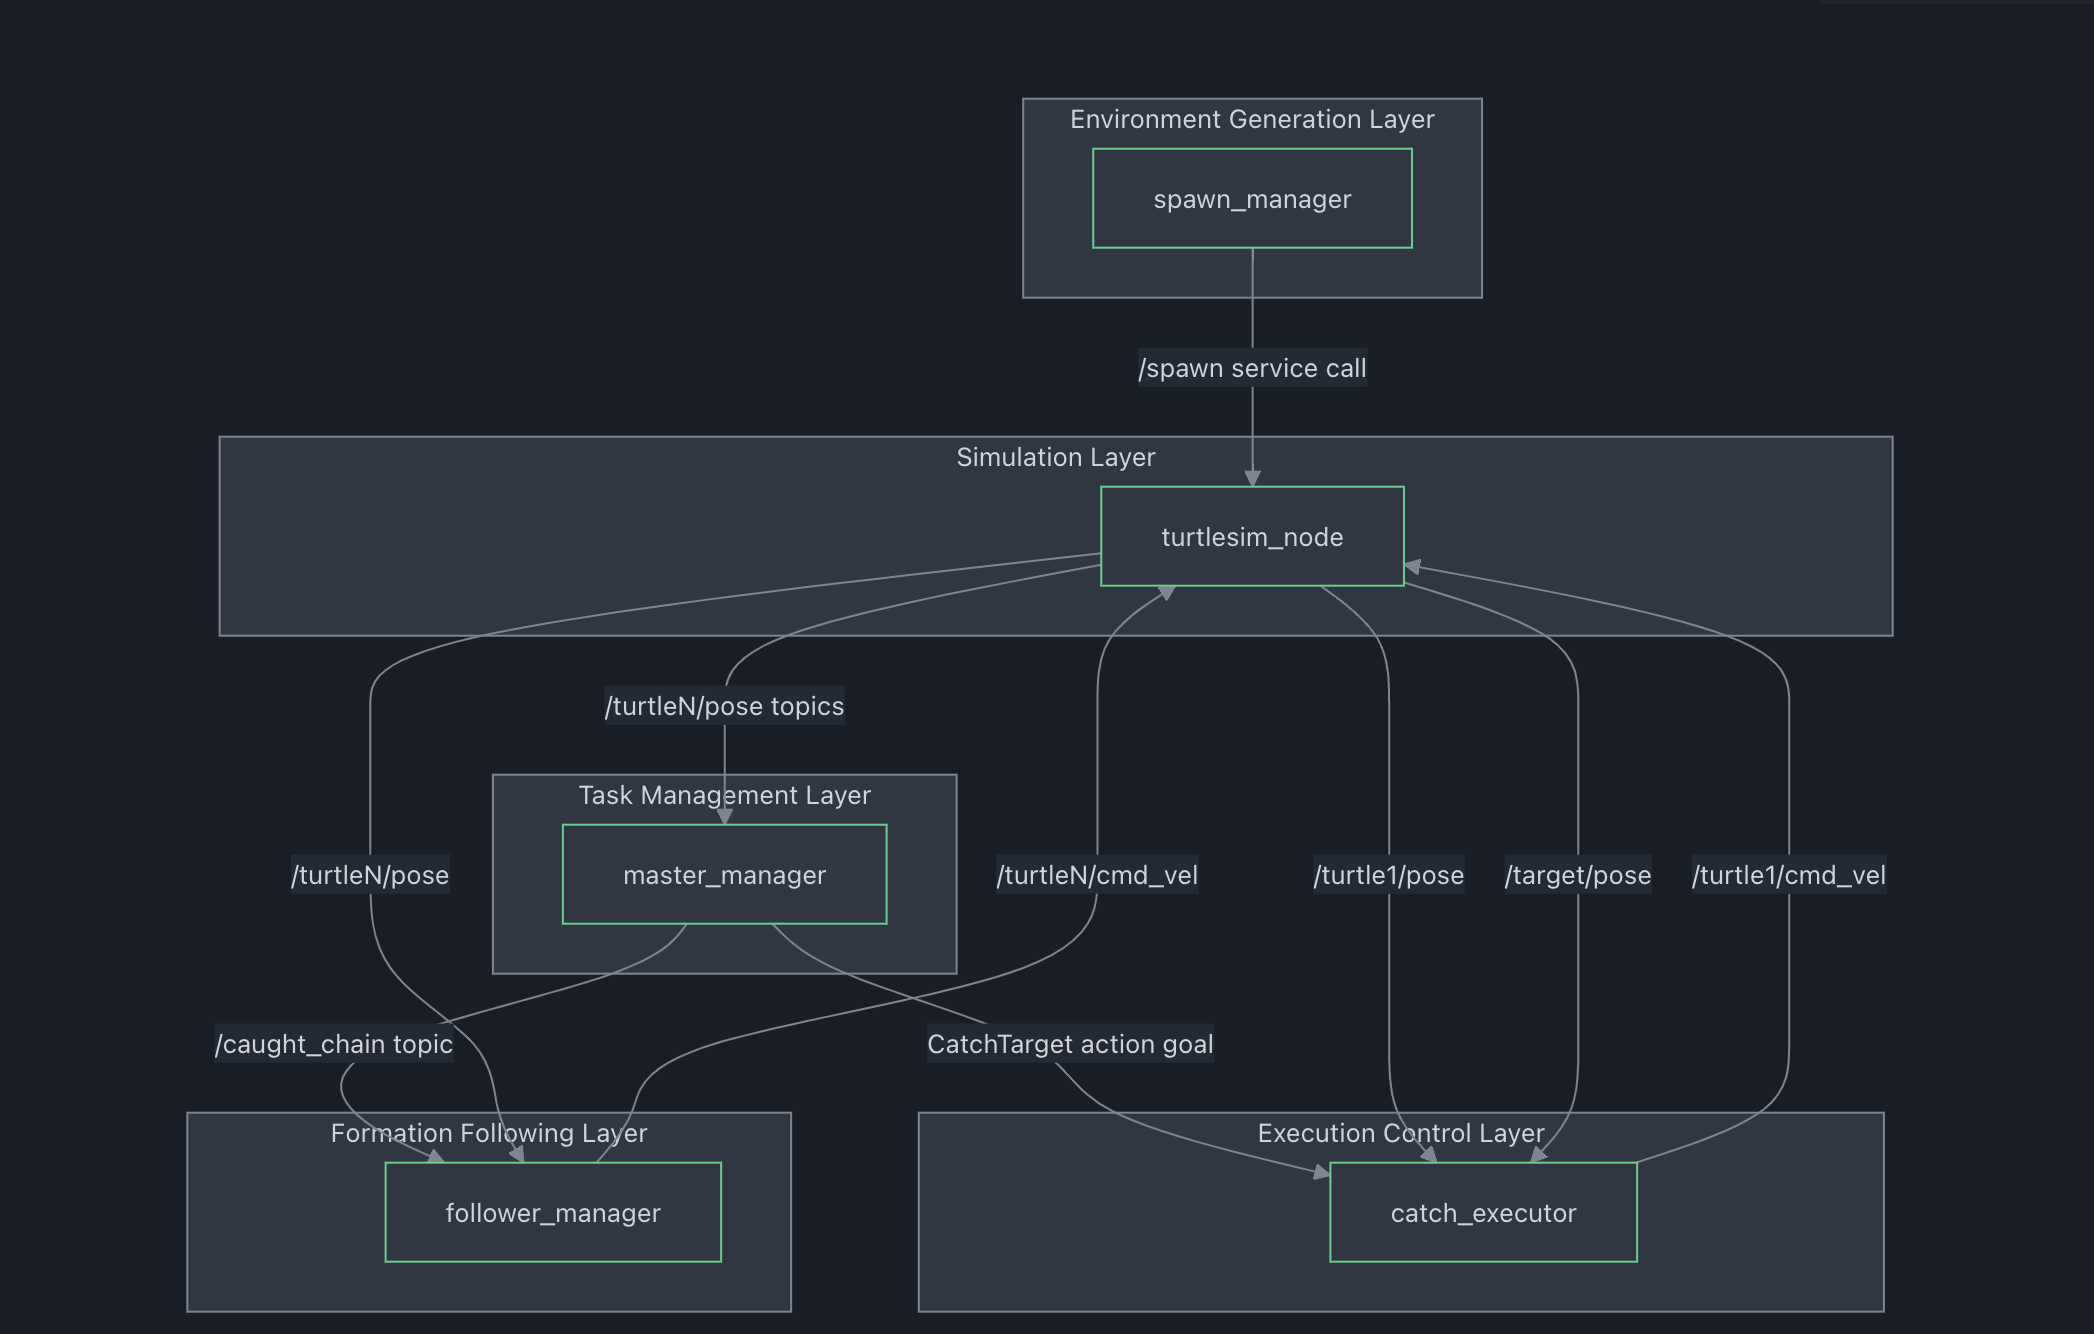
\includegraphics[width=0.85\linewidth]{System Architecture Diagram.png}
\caption{System Architecture Diagram}
\label{fig:architecture}
\end{figure}

\subsection{Node Communication Diagram}

Figure~\ref{fig:communication} shows the communication relationships between all nodes.

\begin{figure}[H]
\centering
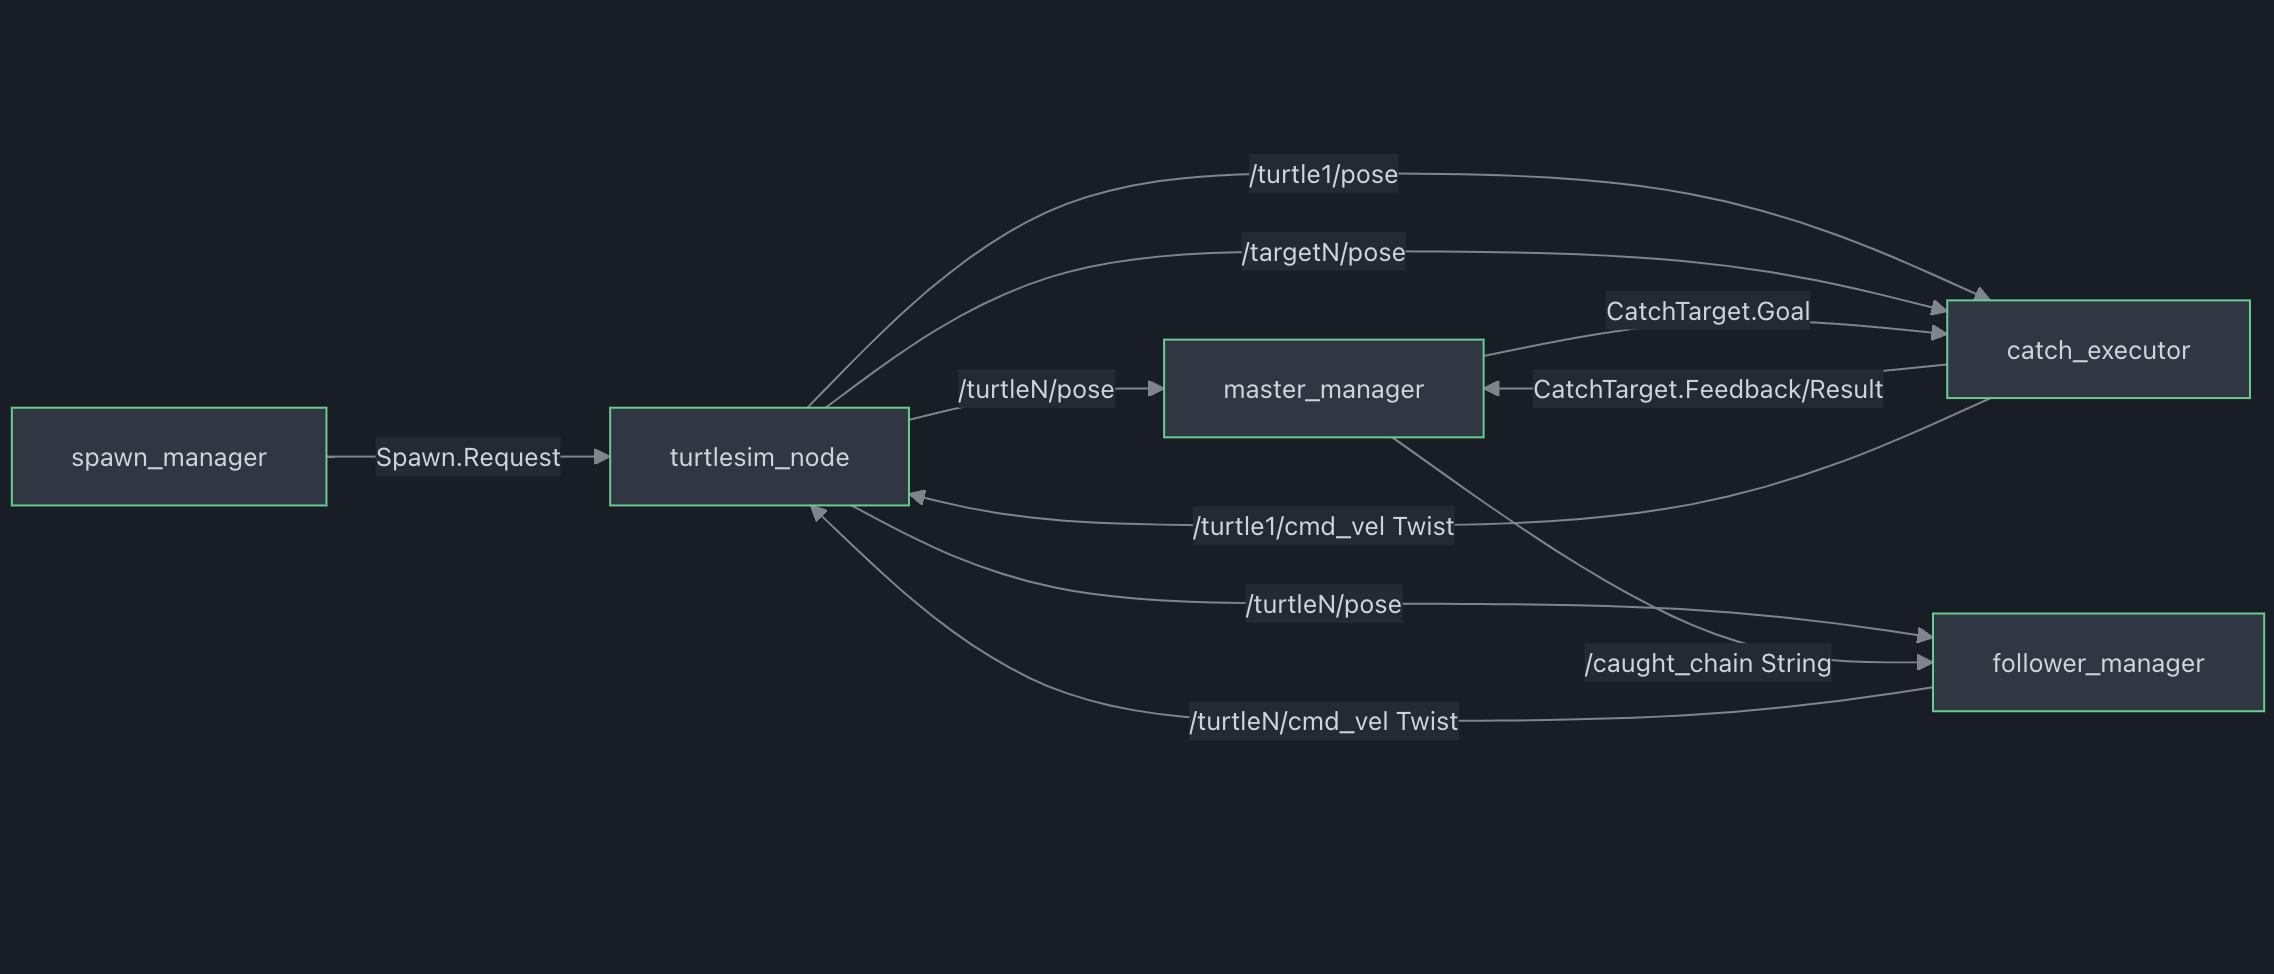
\includegraphics[width=0.95\linewidth]{Node Communication Diagram.png}
\caption{Node Communication Diagram}
\label{fig:communication}
\end{figure}

\subsection{Component Descriptions}

\subsubsection{Custom Action Interface: CatchTarget}

The \texttt{CatchTarget} action defines the communication contract between the task manager and the executor. Its goal specifies the target turtle name; its result confirms success and the caught turtle's identity; its feedback reports the remaining distance in real time. This interface is the foundation of the action-based task execution pattern in the system.

\subsubsection{Spawn Manager}

The \texttt{spawn\_manager} node periodically calls the \texttt{/spawn} service to create new turtles at random positions within the canvas. It handles duplicate names gracefully by scanning existing topics on startup and auto-incrementing indices when spawn requests are rejected. This ensures the system always has fresh targets to pursue.

\subsubsection{Master Manager}

The \texttt{master\_manager} node serves as the system brain. It auto-discovers turtles by scanning pose topics, maintains a registry of all known turtles with their caught/uncaught status, and periodically selects the nearest uncaught target. It dispatches \texttt{CatchTarget} goals to the executor and handles results---updating the caught chain upon success, or placing failed targets on a temporary cooldown.

A key design feature is the \textbf{preemption mechanism with hysteresis}: while a catch goal is in flight, the master manager continuously re-evaluates whether a closer target has appeared. A switch occurs only when the new target is closer by at least a configurable margin (default 1.0\,m). This prevents rapid flip-flopping between two nearly equidistant targets.

\subsubsection{Catch Executor}

The \texttt{catch\_executor} node implements the Action Server for \texttt{catch\_target}. It drives the master turtle toward the designated target using a turn-then-drive control strategy: first rotate to face the target, then move forward while applying proportional angular correction.

It enforces \textbf{single-goal serialization}---rejecting new goals while one is in progress---to prevent conflicting velocity commands. It also protects against stuck goals with total-timeout (30\,s) and no-pose-timeout (5\,s) mechanisms.

Figure~\ref{fig:catchflow} illustrates the internal control flow of the catch executor.

\begin{figure}[H]
\centering
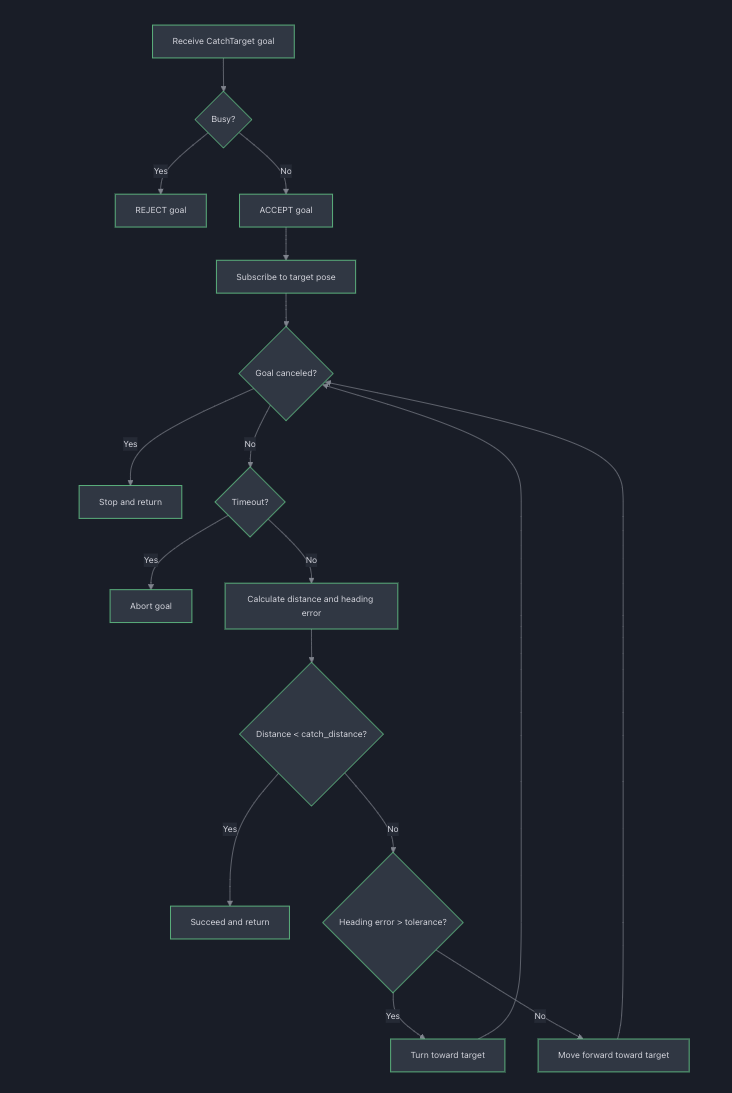
\includegraphics[width=0.75\linewidth]{Catch Executor Control Flow.png}
\caption{Catch Executor Control Flow}
\label{fig:catchflow}
\end{figure}

\subsubsection{Follower Manager}

The \texttt{follower\_manager} node receives the caught chain via the \texttt{/caught\_chain} topic and controls each caught turtle to follow its predecessor. The first caught turtle follows the master; each subsequent turtle follows the one before it. A proportional control law with a distance threshold ensures followers maintain a safe gap without colliding or oscillating.

Figure~\ref{fig:followerchain} shows the follower chain structure.

\begin{figure}[H]
\centering
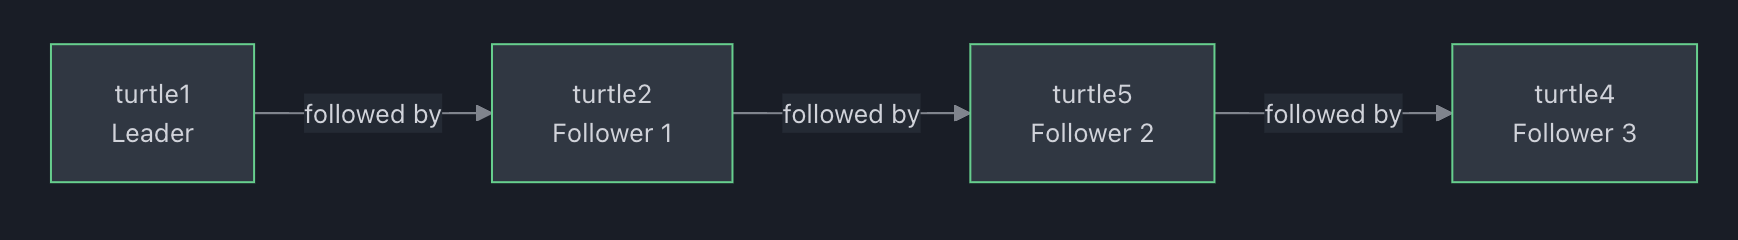
\includegraphics[width=0.7\linewidth]{Follower Chain Diagram.png}
\caption{Follower Chain Diagram}
\label{fig:followerchain}
\end{figure}

\subsubsection{Utility Modules}

Two shared utility modules support the entire system. The \texttt{utils} module provides geometric helper functions (angle normalization, distance calculation, clamping). The \texttt{turtle\_registry} module maintains a centralised state table of all turtles with query methods for uncaught targets and nearest-neighbour selection.

\end{homeworkProblem}


%=============================================================================
% Chapter 3: Component Contributions to Objectives
%=============================================================================
\begin{homeworkProblem}[3]
\section{Chapter 3: Component Contributions to Project Objectives}

This chapter explains how each component contributes to the project objectives outlined in Chapter~1.

\subsection{CatchTarget Action Interface}

This interface directly enables \textbf{O2} (Action-Based Task Execution). By using ROS2 Actions rather than simple services or topics, the system gains structured goal--feedback--result semantics, cancellation support, and the ability to monitor long-running tasks. The feedback channel (reporting remaining distance) allows the master manager to make informed preemption decisions, while the result channel provides unambiguous success/failure reporting.

\textbf{Design Rationale}: Actions were chosen over services because pursuit is a long-running task (several seconds) that requires periodic feedback. A service call would block the caller and provide no mid-flight status, whereas Actions support asynchronous goal dispatch, real-time feedback, and explicit cancellation.

\subsection{Spawn Manager}

This node directly implements \textbf{O3} (Dynamic Environment Generation). Without continuous spawning, the system would quickly exhaust its targets and halt. The robustness features---startup topic scanning and duplicate name handling---ensure the node can run indefinitely without manual intervention, also supporting \textbf{O5} (Robust System Design).

\textbf{Implementation Detail}: On startup, the node scans existing \texttt{/turtleN/pose} topics via a regular expression to determine the next safe index, preventing name collisions when the node restarts while turtles already exist:

\begin{verbatim}
_TURTLE_NAME_RE = re.compile(r'^/turtle(\d+)/pose$')

max_idx = 1
for topic_name, _types in self.get_topic_names_and_types():
    match = _TURTLE_NAME_RE.match(topic_name)
    if match:
        max_idx = max(max_idx, int(match.group(1)))
self._next_index = max(configured_start, max_idx + 1)
\end{verbatim}

If a spawn request is rejected (e.g., name already exists), the node auto-increments the index and retries on the next tick, avoiding infinite loops through a consecutive-failure counter.

\subsection{Master Manager}

This node is central to \textbf{O1} (Autonomous Target Discovery and Pursuit) and \textbf{O2} (Action-Based Task Execution). The auto-discovery mechanism eliminates the need for explicit hand-off between the spawn manager and the master manager. The nearest-target selection logic ensures the master always pursues the most efficient target. The preemption mechanism with hysteresis and the failure cooldown both contribute to \textbf{O5} by preventing oscillation and pathological retry loops.

\textbf{Dynamic Decision Making}: The master manager operates on a continuous decision loop (0.5\,s period). Even while a goal is in flight, it re-evaluates the target landscape. This dynamic decision-making ensures the system adapts to a changing environment rather than being locked into a suboptimal initial choice.

\textbf{Preemption with Hysteresis}: The core preemption logic compares the current target distance against a candidate target distance, applying a configurable margin to prevent flip-flopping:

\begin{verbatim}
margin = float(self.get_parameter('preempt_margin').value)
if new_dist + margin >= cur_dist:
    return  # not worth switching

self._preempting = True
cancel_future = self._goal_handle.cancel_goal_async()
\end{verbatim}

The margin acts as a hysteresis band: a switch occurs only when the new target is closer by at least \texttt{margin} meters (default 1.0\,m). This prevents rapid oscillation between two nearly equidistant targets.

\textbf{Failure Cooldown}: When a goal fails (rejected, aborted, or exception), the target is placed on a temporary cooldown list, excluded from candidate selection until the cooldown expires:

\begin{verbatim}
def _mark_failed(self, target_name):
    cooldown = float(self.get_parameter('failure_cooldown_sec').value)
    self._failed_until[target_name] = time.monotonic() + cooldown
\end{verbatim}

This prevents the system from repeatedly attempting to catch a stuck or unreachable target.

\textbf{Action Client Management}: The master manager manages the full lifecycle of each action goal: dispatch, feedback monitoring, result handling, and cancellation for preemption. This demonstrates proper use of the ROS2 Action client pattern.

\subsection{Catch Executor}

This node directly implements \textbf{O2} (Action-Based Task Execution) by providing the physical pursuit capability. The turn-then-drive control strategy produces clear, visually understandable pursuit behaviour. The single-goal serialization mechanism prevents conflicting velocity commands from multiple concurrent goals, while the timeout handling contributes to \textbf{O5} by detecting and recovering from stuck situations.

\textbf{Single-Goal Serialization}: A threading lock ensures only one goal executes at a time:

\begin{verbatim}
def _on_goal(self, _goal_request):
    if self._busy:
        return GoalResponse.REJECT
    return GoalResponse.ACCEPT

def _try_acquire_busy(self):
    with self._busy_lock:
        if self._busy:
            return False
        self._busy = True
        return True
\end{verbatim}

This prevents race conditions where two concurrent goals would publish conflicting velocity commands to the same turtle.

\textbf{Turn-Then-Drive Control}: The controller first rotates to face the target, then moves forward while applying proportional angular correction. The heading error is computed via angle normalisation:

\begin{verbatim}
target_angle = utils.angle_to(master_pose.x, master_pose.y,
                              target_pose.x, target_pose.y)
heading_err = utils.normalize_angle(target_angle - master_pose.theta)

if abs(heading_err) > angle_tolerance:
    twist.angular.z = utils.clamp(
        angular_speed * utils.sign(heading_err),
        -max_angular_speed, max_angular_speed)
else:
    twist.linear.x = linear_speed
\end{verbatim}

\textbf{Dual Timeout Protection}: Two independent timeouts guard against stuck goals: a total timeout (30\,s) and a ``no pose received'' timeout (5\,s). If either fires, the goal is aborted and the turtle stops:

\begin{verbatim}
if now - start_time > goal_timeout_sec:
    self._publish_zero()
    goal_handle.abort()
    return result

if target_pose is None and now - start_time > no_pose_timeout_sec:
    self._publish_zero()
    goal_handle.abort()
    return result
\end{verbatim}

\subsection{Follower Manager}

This node directly implements \textbf{O4} (Chain Formation Following). The chain-based leader assignment---where each follower tracks its predecessor rather than the master directly---produces natural, snake-like movement. The distance threshold and proportional control contribute to \textbf{O5} by preventing collision and oscillation.

\textbf{Chain-Based Leader Assignment}: Each follower tracks its immediate predecessor in the chain, not the master directly:

\begin{verbatim}
for i, follower in enumerate(self._chain):
    leader = self._leader_name if i == 0 else self._chain[i - 1]
\end{verbatim}

This creates a cascade effect: the first caught turtle follows the master, the second follows the first, and so on. The result is a smooth, snake-like formation rather than all followers converging on a single point.

\textbf{Proportional Control with Distance Threshold}: Followers only move when the gap exceeds a threshold, preventing micro-oscillations:

\begin{verbatim}
if dist < follow_distance:
    pub.publish(Twist())  # stop
    continue

twist.linear.x = utils.clamp(
    linear_kp * (dist - follow_distance),
    0.0, linear_speed)
twist.angular.z = utils.clamp(
    angular_kp * angle_err,
    -max_angular_speed, max_angular_speed)
\end{verbatim}

The linear velocity is proportional to the excess distance beyond the threshold, while angular velocity corrects heading error. This produces smooth, stable following behaviour.

\subsection{Utility Modules}

These modules support all objectives by ensuring consistent, correct geometric computations and reliable state management across nodes. Centralising this logic eliminates duplication and reduces the risk of inconsistent implementations.

\textbf{Angle Normalisation}: The \texttt{normalize\_angle} function wraps angles to $[-\pi, \pi]$, essential for correct heading-error computation:

\begin{verbatim}
def normalize_angle(theta):
    while theta > math.pi:
        theta -= 2.0 * math.pi
    while theta < -math.pi:
        theta += 2.0 * math.pi
    return theta
\end{verbatim}

Without this, a heading error of $359^\circ$ would be miscomputed as $359^\circ$ instead of $-1^\circ$, causing the turtle to rotate the long way around.

\subsection{Summary of Component--Objective Mapping}

Table~\ref{tab:mapping} summarises how each component contributes to the project objectives.

\begin{table}[H]
\centering
\caption{Component--Objective Mapping}
\label{tab:mapping}
\begin{tabular}{lccccc}
\toprule
\textbf{Component} & \textbf{O1} & \textbf{O2} & \textbf{O3} & \textbf{O4} & \textbf{O5} \\
\midrule
CatchTarget Action & & $\bullet$ & & & \\
Spawn Manager & & & $\bullet$ & & $\bullet$ \\
Master Manager & $\bullet$ & $\bullet$ & & & $\bullet$ \\
Catch Executor & & $\bullet$ & & & $\bullet$ \\
Follower Manager & & & & $\bullet$ & $\bullet$ \\
Utility Modules & $\bullet$ & $\bullet$ & $\bullet$ & $\bullet$ & $\bullet$ \\
\bottomrule
\end{tabular}
\end{table}

\end{homeworkProblem}

\end{document}
